%%%%%%%%%%%%%%%%%%%%%%%%%%%%%%%%%%%%%%%%%%%%%%%%%%%%%%%%%%%%%%%%%%%%%%%%%%%%%%%%%%%%%%%%%%%%%%%%%%%%%%%%%%%%%%%%%%%%%%%%%%%%%%%%%%%%%%%%%%%%%%%%%%%%%%%%%%%%%%%%%%%%%%%%%%%%%%%%%%%%%%%%%%%%%%%%%%%%%%%%%%%%%%%%%%%%%%%%%%%%%%%%%%%%%%%%%%%
%%%%%%%%%%%%%%%%%%%%%%%%%%%%%%%%%%%%%%%%%%%%%%%%%%%%%%%%%%%%%%%%%%%%%%%%%%%%%%%%%%%%%%%%%%%%%%%%%%%%%%%%%%%%%%%%%%%%%%%%%%%%%%%%%%%%%%%%%%%%%%%%%%%%%%%%%%%%%%%%%%%%%%%%%%%%%%%%%%%%%%%%%%%%%%%%%%%%%%%%%%%%%%%%%%%%%%%%%%%%%%%%%%%%%%%%%%%
%%%%%%%%%%%%%%%%%%%%%%%%%%%%%%%%%%%%%%%%%%%%%%%%%%%%%%%%%%%%%%%%%%%%%%%%%%%%%%%%%%%%%%%%%%%%%%%%%%%%%%%%%%%%%%%%%%%%%%%%%%%%%%%%%%%%%%%%%%%%%%%%%%%%%%%%%%%%%%%%%%%%%%%%%%%%%%%%%%%%%%%%%%%%%%%%%%%%%%%%%%%%%%%%%%%%%%%%%%%%%%%%%%%%%%%%%%%
\chapter{Introduction}
\label{res:ch:Introduction}

The determination and quantification of the quality of the jet transverse momentum measurement is of crucial interest for many analyses with jet final states, \eg the measurement of the dijet cross section~\cite{bib:CMS:QCD_measurements} or \ttbar production cross sections~\cite{bib:CMS:TopCrossSection_8TeV}. 
Also searches for physics beyond the standard model with missing transverse momentum, \PTm, in the final state need a good knowledge of \PTm originating from wrongly measured jets~\cite{bib:CMS:RA2_8TeV,bib:CMS:MT2_8TeV,bib:CMS:AlphaT_8TeV}.
For analyses relying on information from simulation it is very important to correct the simulated resolution to the resolution actually present in data.
Therefore, scale factors will be presented to adjust the resolution in simulation to the resolution of the real detector.  
  
In the following sections, a data-based method to measure the jet \pt resolution in \GAMJET events will be presented. 
A similar method was already accomplished in earlier analyses~\cite{bib:CMS:JERCPaper_2011,bib:CMS-AN-2010-076,bib:CMS-AN-2010-141,bib:CMS-AN-2011-004} of 7\tev data.  
It is further developed here and applied to 8\tev data.

The method is based on the transverse momentum balance in the \GAMJET system. 
It takes advantage of the high resolution of the electromagnetic calorimeter and hence the excellent measurement of the photon energy and momentum.
Without initial and final state radiation, the photon and the jet are balanced in the transverse plane. 
Thus, measuring the photon \pt with high accuracy leads to an estimate of the true jet transverse momentum offering a possibility to quantify the resolution of jet \pt measurements.


%%%%%%%%%%%%%%%%%%%%%%%%%%%%%%%%%%%%%%%%%%%%%%%%%%%%%%%%%%%%%%%%%%%%%%%%%%%%%%%%%%%%%%%%%%%%%%%%%%%%%%%%%%%%%%%%%%%%%%%%%%%%%%%%%%%%%%%%%%%%%%%%%%%%%%%%%%%%%%%%%%%%%%%%%%%%%%%%%%%%%%%%%%%%%%%%%%%%%%%%%%%%%%%%%%%%%%%%%%%%%%%%%%%%%%%%%%%
%%%%%%%%%%%%%%%%%%%%%%%%%%%%%%%%%%%%%%%%%%%%%%%%%%%%%%%%%%%%%%%%%%%%%%%%%%%%%%%%%%%%%%%%%%%%%%%%%%%%%%%%%%%%%%%%%%%%%%%%%%%%%%%%%%%%%%%%%%%%%%%%%%%%%%%%%%%%%%%%%%%%%%%%%%%%%%%%%%%%%%%%%%%%%%%%%%%%%%%%%%%%%%%%%%%%%%%%%%%%%%%%%%%%%%%%%%%
%%%%%%%%%%%%%%%%%%%%%%%%%%%%%%%%%%%%%%%%%%%%%%%%%%%%%%%%%%%%%%%%%%%%%%%%%%%%%%%%%%%%%%%%%%%%%%%%%%%%%%%%%%%%%%%%%%%%%%%%%%%%%%%%%%%%%%%%%%%%%%%%%%%%%%%%%%%%%%%%%%%%%%%%%%%%%%%%%%%%%%%%%%%%%%%%%%%%%%%%%%%%%%%%%%%%%%%%%%%%%%%%%%%%%%%%%%%
\chapter{General approach of the resolution measurement using photon+jet events}
\label{res:ch:GeneralApproach}

The jet transverse momentum resolution is defined as the standard deviation of the jet transverse momentum response distribution with the response defined as the ratio of the reconstructed to the true jet transverse momentum 
\begin{equation}\label{res:eq:responseFormula}
\mathcal{R} =  \frac{\pt^{\text{reco. jet}}}{\pt^{\text{gen. jet}}}.
\end{equation}
The transverse momentum of the generator-level jet is hereby defined as the sum of all particles' transverse momenta that are clustered into the jet cone.
It can differ to the momentum of the original final state quark or gluon by out-of-cone showering effects.
Out-of-cone showering refers to particles from the hadronisation process that are not clustered into the jet cone.
Throughout the following sections, the jet transverse momentum resolution will be abbreviated JER\footnote{This abbreviation is a historical relic from electron-position collider experiments where JER refered to jet energy resolution. FIXME - is this correct}.

\mbox{Figure~\ref{res:fig:TypicalResponse}} shows a typical response distribution for jets in the barrel region.
\begin{figure}[b]
  \centering
      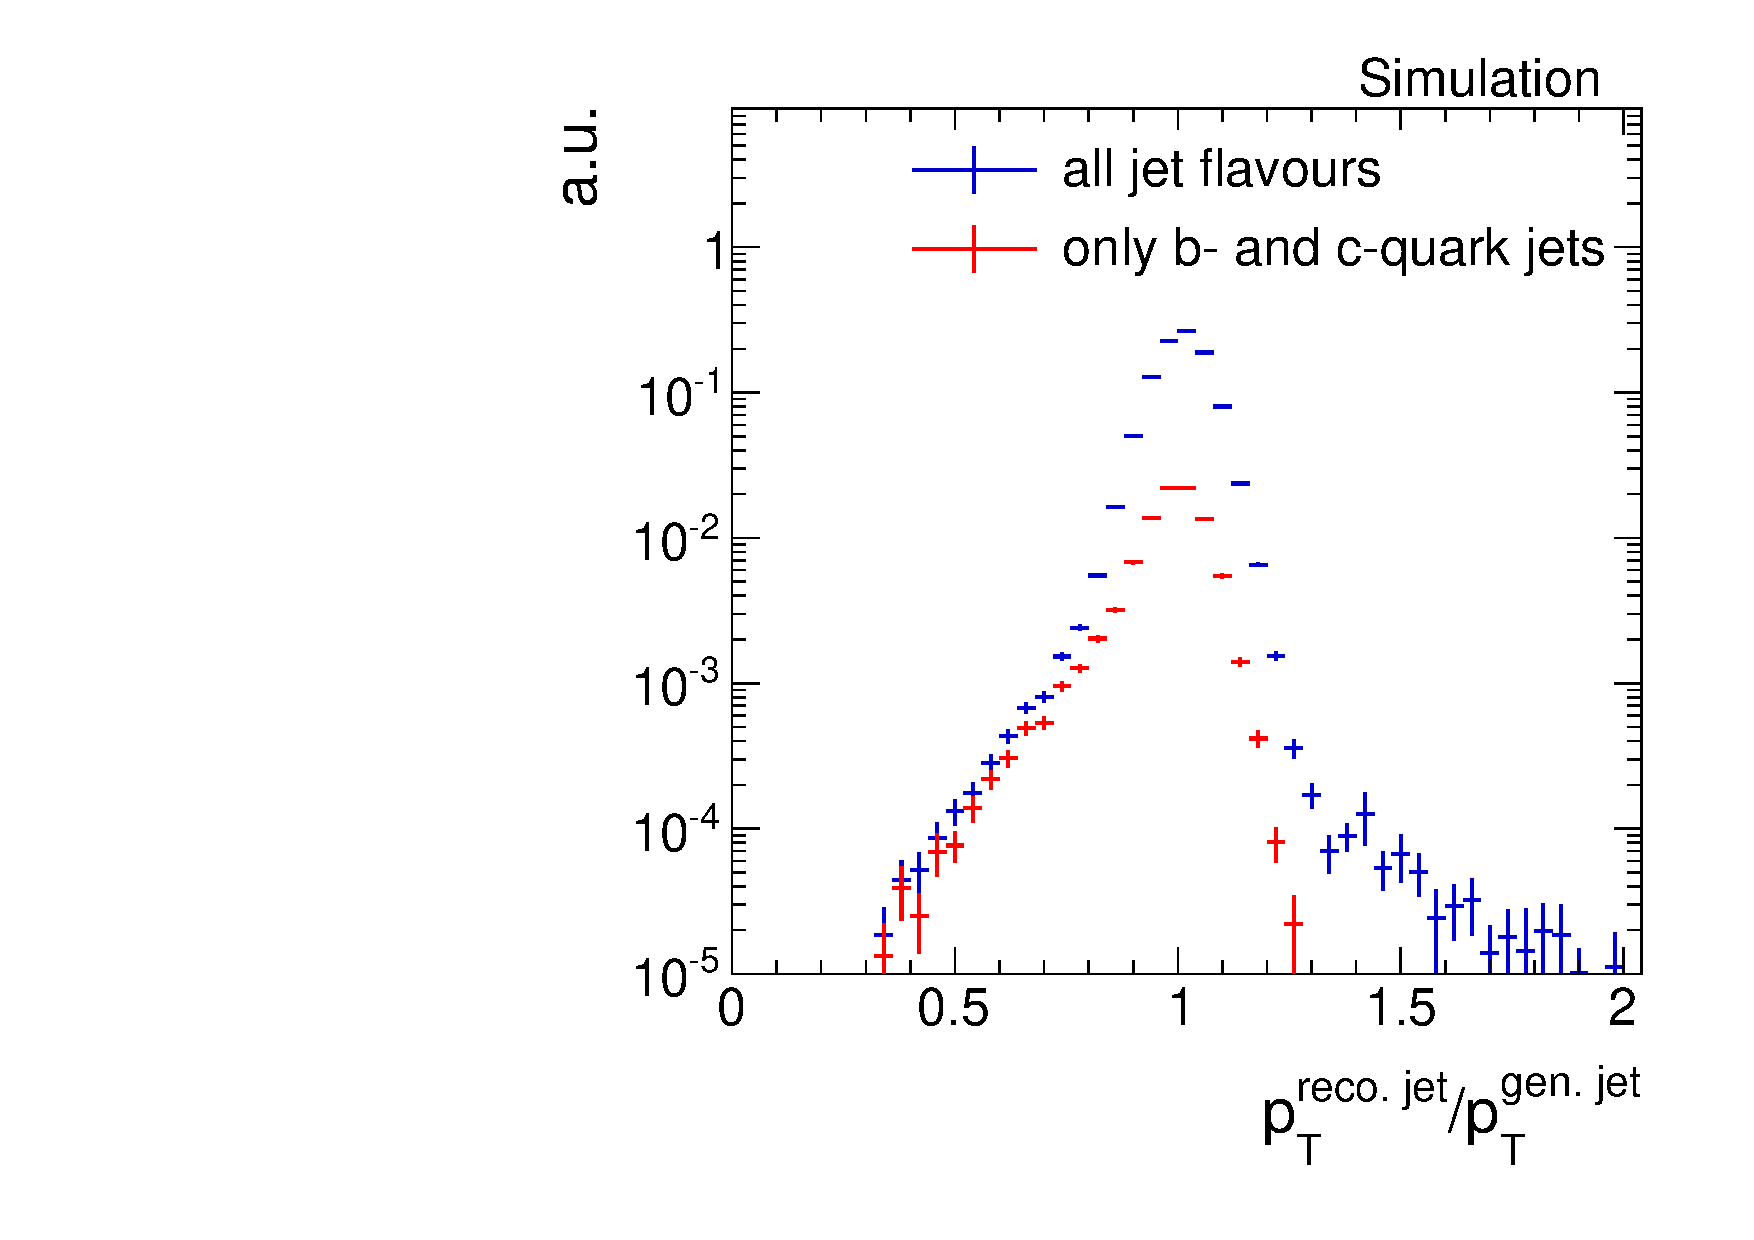
\includegraphics[width=0.49\textwidth]{figures/resolution/generalApproach/intrinsicExampleContributionofBCQuarks.pdf}
  \caption{Number of events over $\frac{\pt^{\text{reco. jet}}}{\pt^{\text{gen. jet}}}$ from a simulated \GAMJET sample. 
           The black dots show the contribution by c- and b-quark jets where the left tail originating from semi-leptonic decays of heavy quarks can be seen.}  
  \label{res:fig:TypicalResponse}
\end{figure}
The core of the response distribution shows a Gaussian behavior whereas the tails deviate from that functional form.
%The Gaussian behaviour originates from the poissian fluctionation of the number of secondary particles that are released in the calorimeters.
%This is then transferred to the momentum measurment with pt = e*x.
FIXME: The Gaussian behaviour originates for charged particles contained in the jet, for which the momentum is determined by the curvature of the particles' trajectories, from the distribution of the scattering angle. 
For neutral particles clustered into a jet, the Gaussian is p and the Poissoian error for neutral hadrons where the momenntum is measured with the help of the energy m,easurement in the calorimeter.

Physical reasons for the low response tail are inter alia semi-leptonic decays of heavy quarks where the neutrino cannot be detected and the reconstructed transverse momentum of the jet is too small (see \mbox{Fig.~\ref{res:fig:TypicalResponse}}). 
Only since neutrinos are included into the generator-level jet, this effect is visible.
Some instrumental effects, such as a non-linear response of the calorimeter, inhomogeneities of the detector material and electronic noise can contribute to both tails, 
others, like dead calorimeter channels only contribute to the left tail. 
The resolution is therefore determined using only the core of the distribution to avoid the coverage of non-Gaussian tails.
The resolution is thus defined as the standard deviation of the 99\% truncated response histogram devided by the mean of the histogram:

\begin{equation*}\label{res:eq:resolutionFormula}
\text{JER} = \frac{\sigma_{99\%}}{\mu_{99\%}}.
\end{equation*}

The determination of the 99\% range of the histogram is done in several steps. 
First the mean of the core is found via a Gaussian fit to the histogram in a 2$\sigma$ range\footnote{The 2$\sigma$ range is defined as the range [$\mu - 2\sigma$,$\mu + 2\sigma$].}. 
This procedure is done in three iteration steps.
Then, a symmetric interval around this mean is determined with its integral equal to 99\% of the integral of the full histogram. 

%The division by the mean is done to make the resolution measurement more insensitive to a variation of the jet energy scale (= mean of the response distribution)
%which has also an effect on the measured width of the distribution. 
%because response distributions with a scale smaller than one are typically narrower while distributions with scales larger than one are broader.

The evaluation of the response distribution as reconstructed over generated jet transverse momentum (\mbox{Eq.~\eqref{res:eq:responseFormula}})
is only possible for simulated events where generator-level information is accessible. 
A determination of the resolution in data, however, has to rely on a different approach.\\

The main idea of a resolution measurement using \GAMJET events is based on the transverse momentum balance of the \GAMJET system and the excellent electromagnetic calorimeter resolution
(which was estimated between 1.1 \% and 3.8\% in the barrel region for photons for $\sqrt{s}=8\tev$ data~\cite{bib:CMS:PhotonResolution_8TeV}).

In Fig~\ref{res:fig:FeynmanDiagrams}, all tree-level processes contributing to an event topology with one photon and one jet in the final state are depicted. 
\begin{figure}[b]
  \centering
      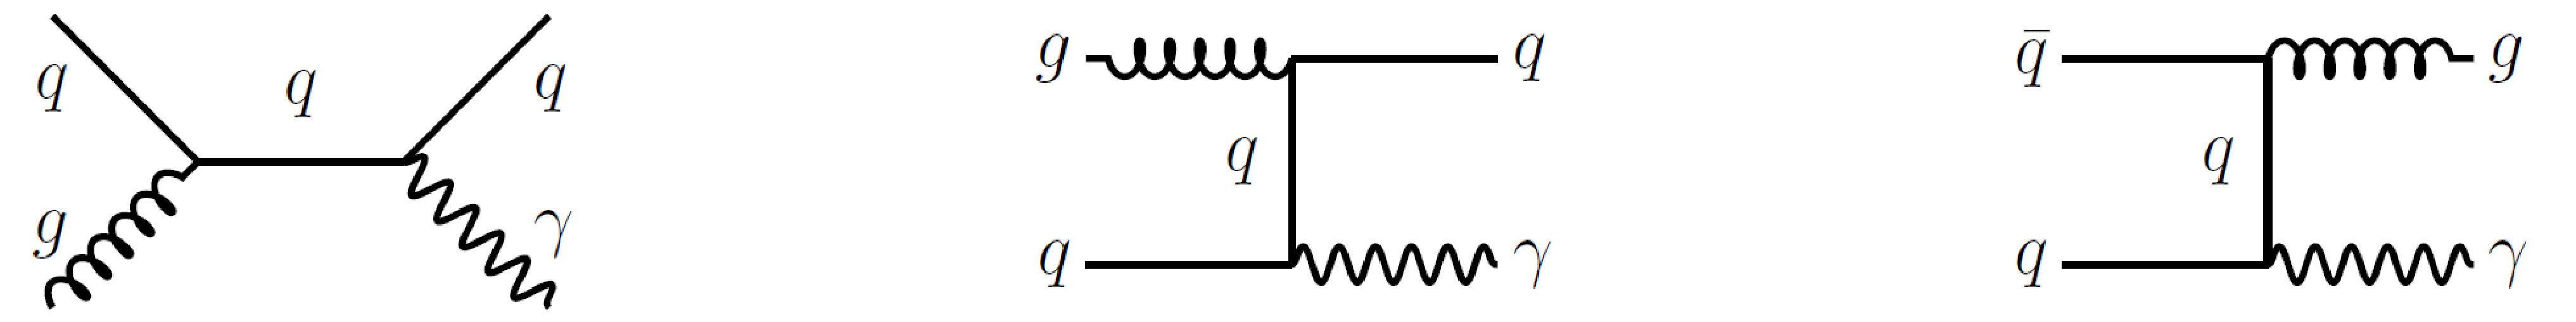
\includegraphics[width=0.99\textwidth]{figures/resolution/generalApproach/FeynmanDiagram.pdf}
  \caption{Tree-level Feynman diagrams of processes at the LHC in pp collisions with one photon and one jet in the final state.}  
  \label{res:fig:FeynmanDiagrams}
\end{figure}
Due to momentum conversation, the jet and the photon are back to back in the transverse plane, and therefore, $\ptvec^{\,\gamma} = -\ptvec^{\,\text{jet}}$. 
Because of the good resolution of the electromagnetic calorimeter, photon energies can be very well measured 
and thus can serve as an excellent estimator for the true jet energy.


Unfortunately, such clean events are very rare processes, and usually, the momentum balance is spoiled by initial and final state radiation, which lead to further jets in the event 
(see \mbox{Fig. \ref{res:fig:FeynmanDiagramsWithRadiation}}). 
However, in order to select events that are balanced to a large extent, a lower bound 
on the angular distance in the transverse plane between the photon and the jet with the highest transverse momentum (leading jet) is required ($\Delta\Phi>2.95\,\unit{rad}$). 

Additionally, the variable 
\begin{equation*}\label{res:eq:alphaDef}
\alpha \doteq \frac{\pt^{\text{\nth{2} reco jet}}}{\pt^{\gamma}}
\end{equation*} 
is defined as a measure of further jet activity in an event. 
It is, however, not sufficient to require only an upper bound on $\alpha$. 
Instead, the jet energy resolution is measured in bins of $\alpha$ (with max($\alpha$) = 0.2), 
and the \mbox{extrapolated} value to zero further jet energy ($\alpha=0$) is taken as the measured resolution of the jet energy in the absence of further jets.
\begin{figure}[t]
  \centering
      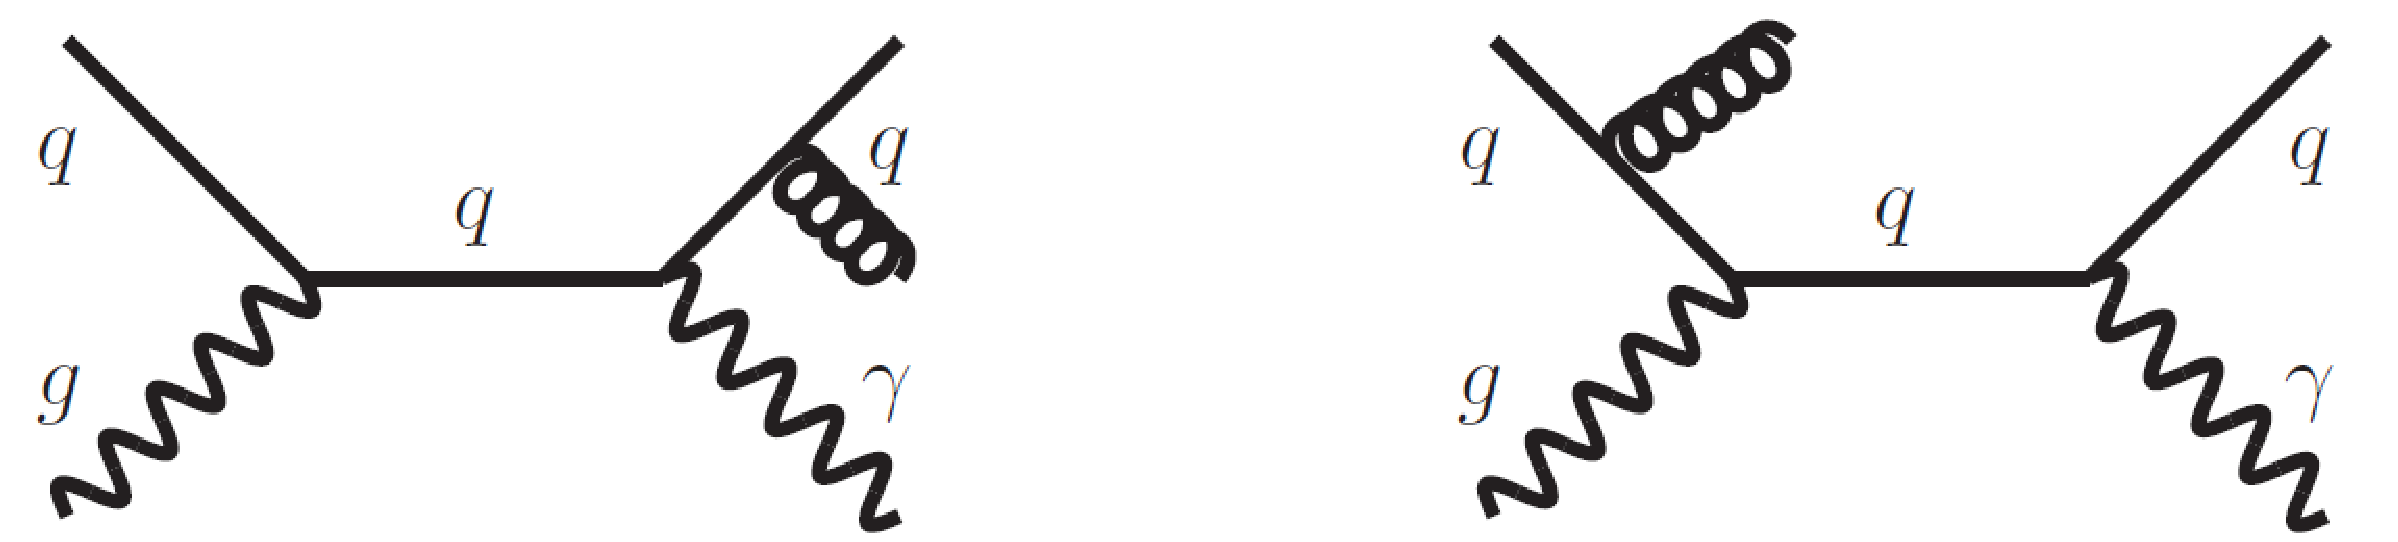
\includegraphics[width=0.60\textwidth]{figures/resolution/generalApproach/FeynmanDiagramsWithRadiation.pdf}
  \caption{Tree-level Feynman diagrams with initial and final state radiation.}  
  \label{res:fig:FeynmanDiagramsWithRadiation}
\end{figure}

Measuring the transverse momentum of the photon instead of taking the generator-level jet \pt leads to the fact that the measured resolution consists out of two parts
\begin{equation*}\label{res:eq:splitting}
\frac{\pt^{\text{reco. jet}}}{\pt^{\gamma}} = \underbrace{\frac{\pt^{\text{reco. jet}}}{\pt^{\text{gen. jet}}}}_{\text{intrinsic}} \cdot \underbrace{\frac{\pt^{\text{gen. jet}}}{\pt^{\gamma}}}_{\text{imbalance}}.
\end{equation*}
The intrinsic part is the resolution of interest which is independent of further jets in the event whereas the imbalance is strongly dependent on $\alpha$.

To extract the intrinsic resolution out of the measured one, the residual imbalance $q^{\prime}$ (the imbalance at $\alpha = 0$) is subtracted from the total resolution in the 
limit of vanishing additional jet activity. 
As that information is only available from simulation, the measured resolution in data is corrected by the residual imbalance taken from the simulated dataset.
%%%%%%%%%%%%%%%%%%%%%%%%%%%%%%%%%%%%%%%%%%%%%%%%%%%%%%%%%%%%%%%%%%%%%%%%%%%%%%%%%%%%%%%%%%%%%%%%%%%%%%%%%%%%%%%%%%%%%%%%%%%%%%%%%%%%%%%%%%%%%%%%%%%%%%%%%%%%%%%%%%%%%%%%%%%%%%%%%%%%%%%%%%%%%%%%%%%%%%%%%%%%%%%%%%%%%%%%%%%%%%%%%%%%%%%%%%%

%%%%%%%%%%%%%%%%%%%%%%%%%%%%%%%%%%%%%%%%%%%%%%%%%%%%%%%%%%%%%%%%%%%%%%%%%%%%%%%%%%%%%%%%%%%%%%%%%%%%%%%%%%%%%%%%%%%%%%%%%%%%%%%%%%%%%%%%%%%%%%%%%%%%%%%%%%%%%%%%%%%%%%%%%%%%%%%%%%%%%%%%%%%%%%%%%%%%%%%%%%%%%%%%%%%%%%%%%%%%%%%%%%%%%%%%%%%
%%%%%%%%%%%%%%%%%%%%%%%%%%%%%%%%%%%%%%%%%%%%%%%%%%%%%%%%%%%%%%%%%%%%%%%%%%%%%%%%%%%%%%%%%%%%%%%%%%%%%%%%%%%%%%%%%%%%%%%%%%%%%%%%%%%%%%%%%%%%%%%%%%%%%%%%%%%%%%%%%%%%%%%%%%%%%%%%%%%%%%%%%%%%%%%%%%%%%%%%%%%%%%%%%%%%%%%%%%%%%%%%%%%%%%%%%%%
\chapter{Datasets and event selection}

The measurement of the jet energy resolution is carried out with \GAMJET data recorded during the year 2012 at the CMS experiment.
The datasets and triggers that are exploitet for this measurement are introduced in the following Section~\ref{res:sec:DatasetsAndTriggers}.
In order to select \GAMJET events that are well suited for the resolution measurement, an event selection is applied on top. % to ensure \GAMJET events that show already the disired back-to-back signatures.
This event selection is described in Section~\ref{res:sec:EventSelection}.

\section{Datasets and triggers}
\label{res:sec:DatasetsAndTriggers}
This analysis exploits several triggers which were active during the year 2012 at the CMS experiment.
Because of the high production cross section of \GAMJET events, especially for low photon \pt, almost all of these triggers were highly prescaled, \ie only a fraction of events were actually recorded when the triggers fired.
All triggers utilised in this measurement are listed in Table~\ref{res:tab:triggers} together with their recorded luminosity.
\renewcommand{\arraystretch}{1.5}
\begin{table}[!hbt]
\centering
\caption{Single photon triggers together with the recorded luminosity taken the time when they were active and the prescales of the triggers into consideration.}
\label{res:tab:triggers}
\makebox[0.99\textwidth]{
\begin{tabular}{lr}
\multicolumn{2}{c}{} \\
\toprule
Trigger                       & Luminosity [\fbinv]   \\
\midrule
HLT\_Photon30\_CaloIdVL\_IsoL & \\
HLT\_Photon50\_CaloIdVL\_IsoL & \\
HLT\_Photon75\_CaloIdVL\_IsoL & \\
HLT\_Photon90\_CaloIdVL\_IsoL & \\
HLT\_Photon135\               & \\
HLT\_Photon150\               & \\
\bottomrule
\multicolumn{2}{c}{} \\
\end{tabular}}
\end{table}  
L1 trigger information should be described her FIXME.
The triggers  require a photon with a certain \pt (as indicated in the name) and, in case of thresholds below \mbox{135\gev} also additional quality and isolation criteria. 
All triggers with threshold below \mbox{150\gev} were prescaled.

The events that are selected by the above mentioned triggers are contained in the datasets listed in Table~\ref{res:tab:datasets}.

\renewcommand{\arraystretch}{1.5}
\begin{table}[!hbt]
\centering
\caption{Single-photon data samples used for the resolution measurement with the contained integrated luminosity.}
\label{res:tab:datasets}
\makebox[0.99\textwidth]{
\begin{tabular}{l r}
\multicolumn{2}{c}{} \\
\toprule
Dataset                                          & Luminosity [\fbinv]   \\
\midrule
 /Photon/Run2012A-22Jan2013-v1/AOD               &  0.876   \\
 /SinglePhoton/Run2012B-22Jan2013-v1/AOD         &  4.412  \\
 /SinglePhoton/Run2012C-22Jan2013-v1/AOD         &  7.055  \\
 /SinglePhotonParked/Run2012D-22Jan2013-v1/AOD   &  7.354  \\ 
\bottomrule
\multicolumn{2}{c}{} \\
\end{tabular}}
\end{table}  





Monte Carlo simulation data was obtained from a flat $\pythia 6$ sample\\ 
\texttt{/G\_Pt-15to3000\_TuneZ2\_Flat\_8TeV\_pythia6/}\\
\texttt{Summer12\_DR53X-PU\_S10\_START53\_V7A-v1/AODSIM}\\
with the events reconstructed with \texttt{CMSSW\_5\_3\_2\_patch5} and the Global Tag \texttt{START53\_V22}.

The simulated events were reweighed to match the physical photon \pt spectrum. 
\mbox{Figure \ref{res:fig:PhotonPtSpectrum}} shows the photon \pt spectrum in simulation before and after the reweighing. 
Due to the flat generation, statistical precision remains high, even in the high photon \pt region.
\begin{figure}[b]
  \centering
      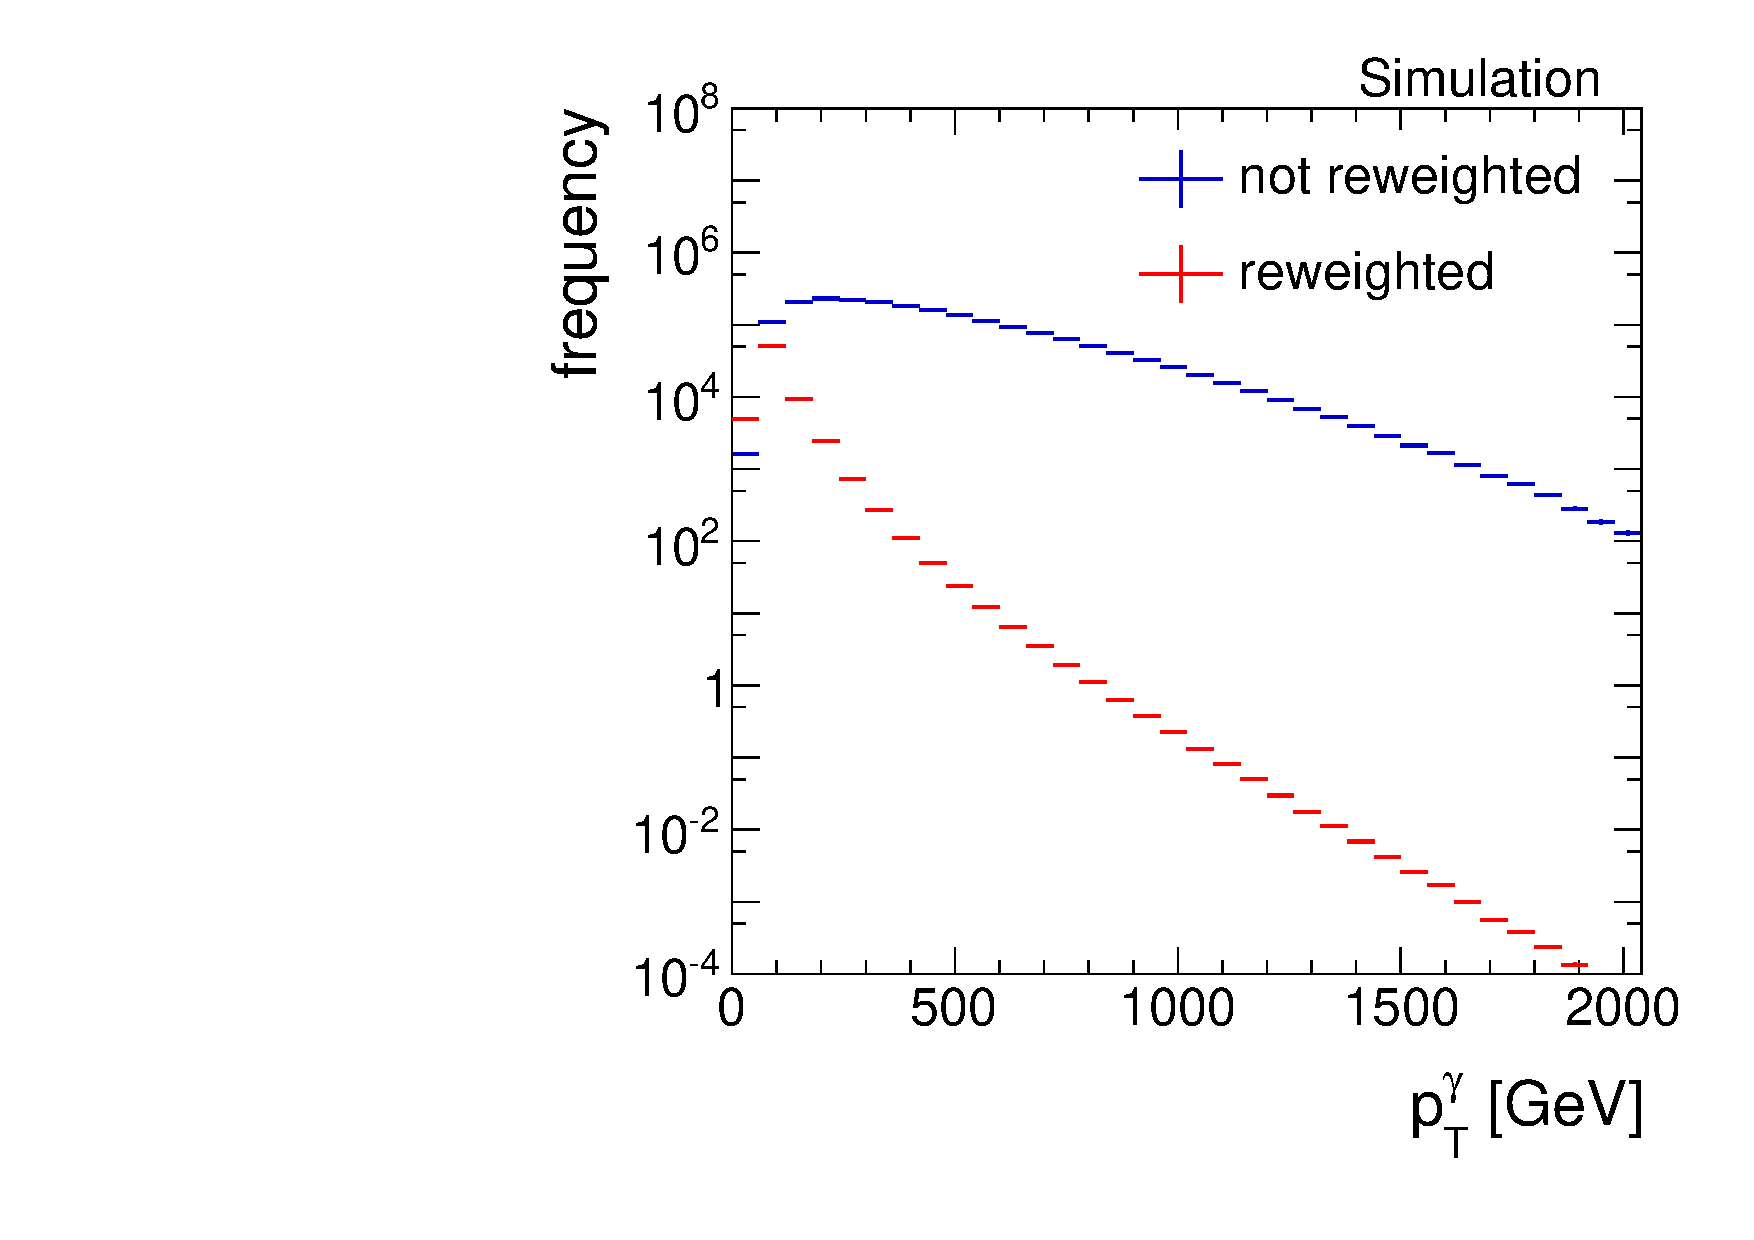
\includegraphics[width=0.49\textwidth]{figures/resolution/eventSelection/PhotonPtComparison_reweighted.pdf} 
  \caption{The photon \pt spectrum before (blue) and after (red) reweighing.}  
  \label{res:fig:PhotonPtSpectrum}
\end{figure}

All simulated samples come with a pileup scenario which does not necessarily match the pileup scenario in data. 
To match the measured distribution of primary vertices, the events are weighted according to their number of primary vertices. 
Because almost all of the used triggers are differently prescaled, the distributions of primary vertices differ among the various events triggered by the corresponding trigger.
Thus the reweighing has to be done separately for the events falling in the photon \pt range of the several triggers (see \mbox{Tab. \ref{res:tab:PhotonPtBins}}).
In \mbox{Fig. \ref{res:fig:PUreweighing}}, a comparison between the number of primary vertices for events with $\pt^{\gamma}>165\gev$ is shown before and after the reweighing. 
For all other triggers the comparison can be found in \mbox{appendix \ref{res:app:PUhistos}}.

\begin{figure}[tbp]
 \centering
    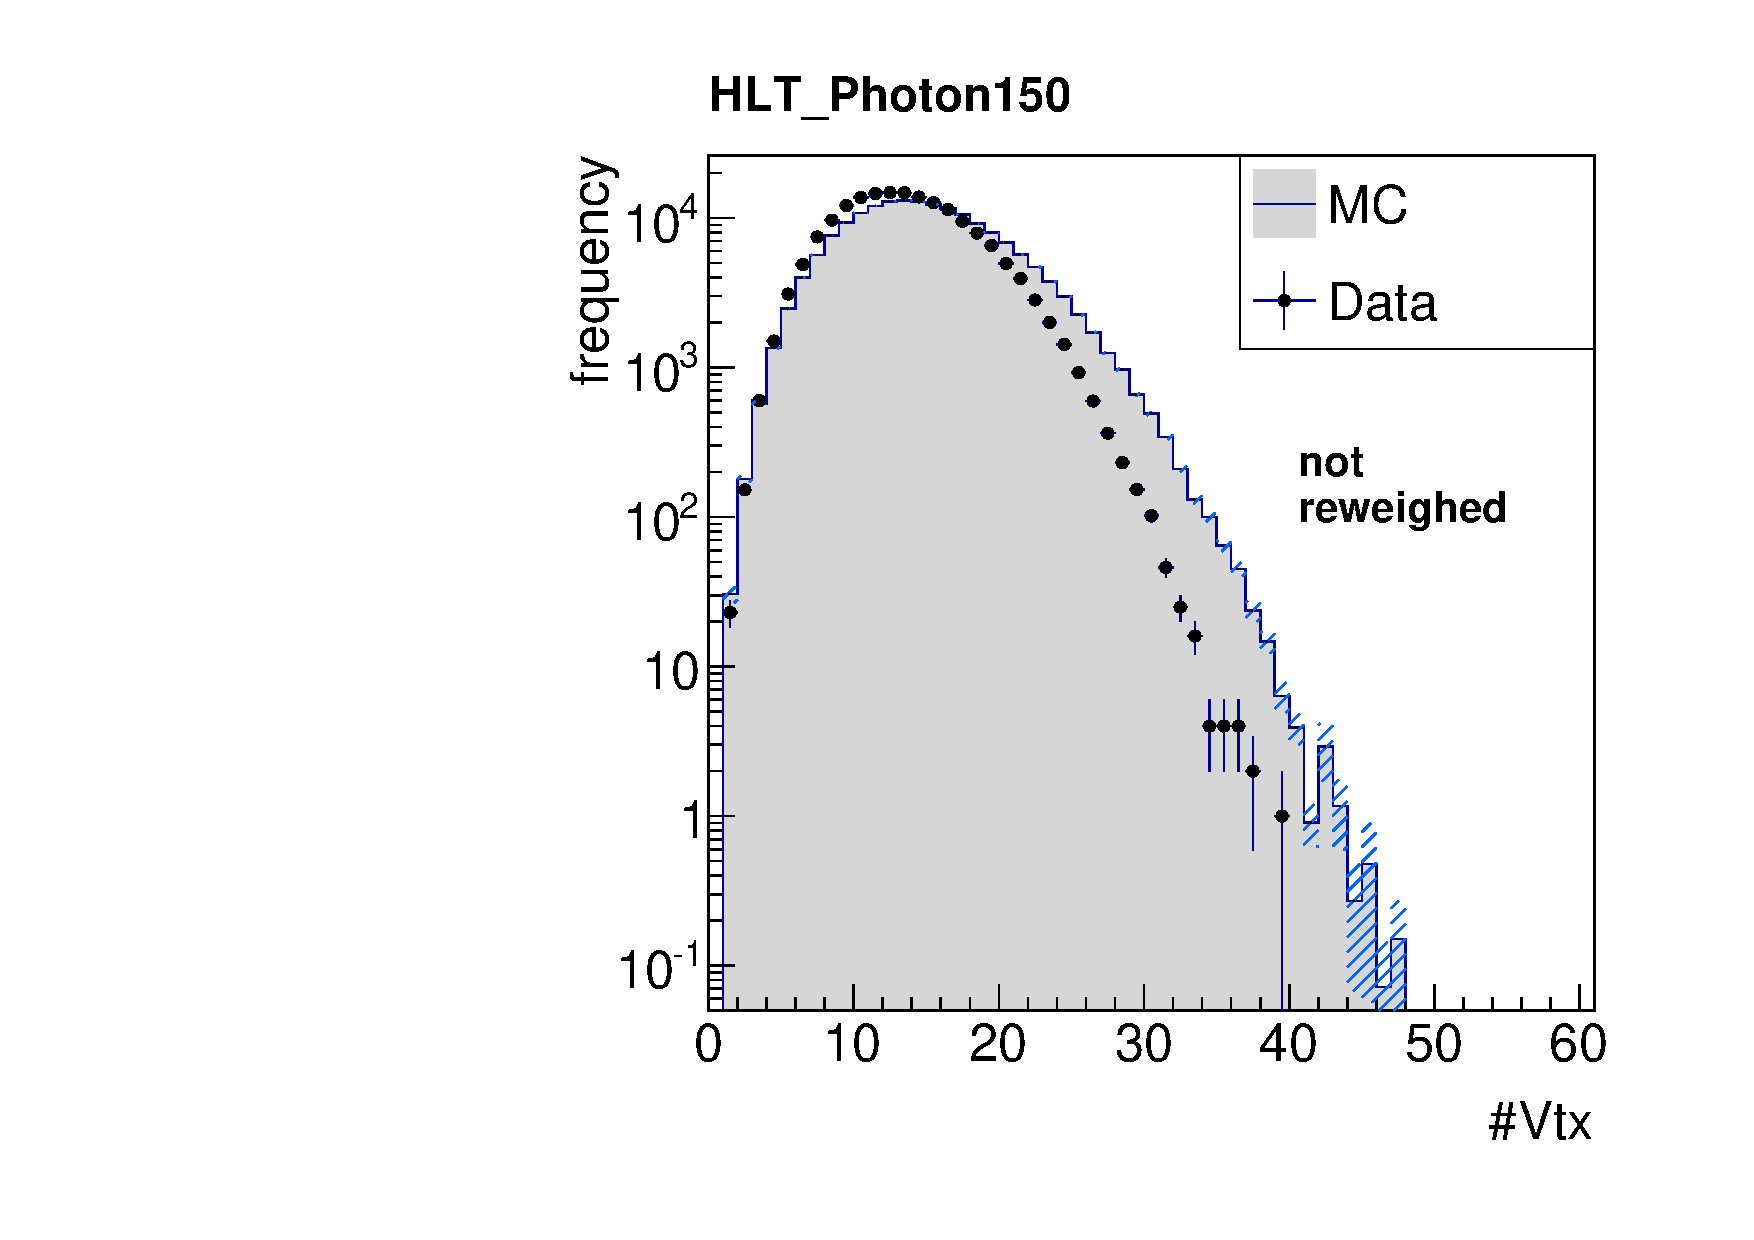
\includegraphics[width=0.49\textwidth]{figures/resolution/eventSelection/NVtxComparisonWoWeights6.pdf}
    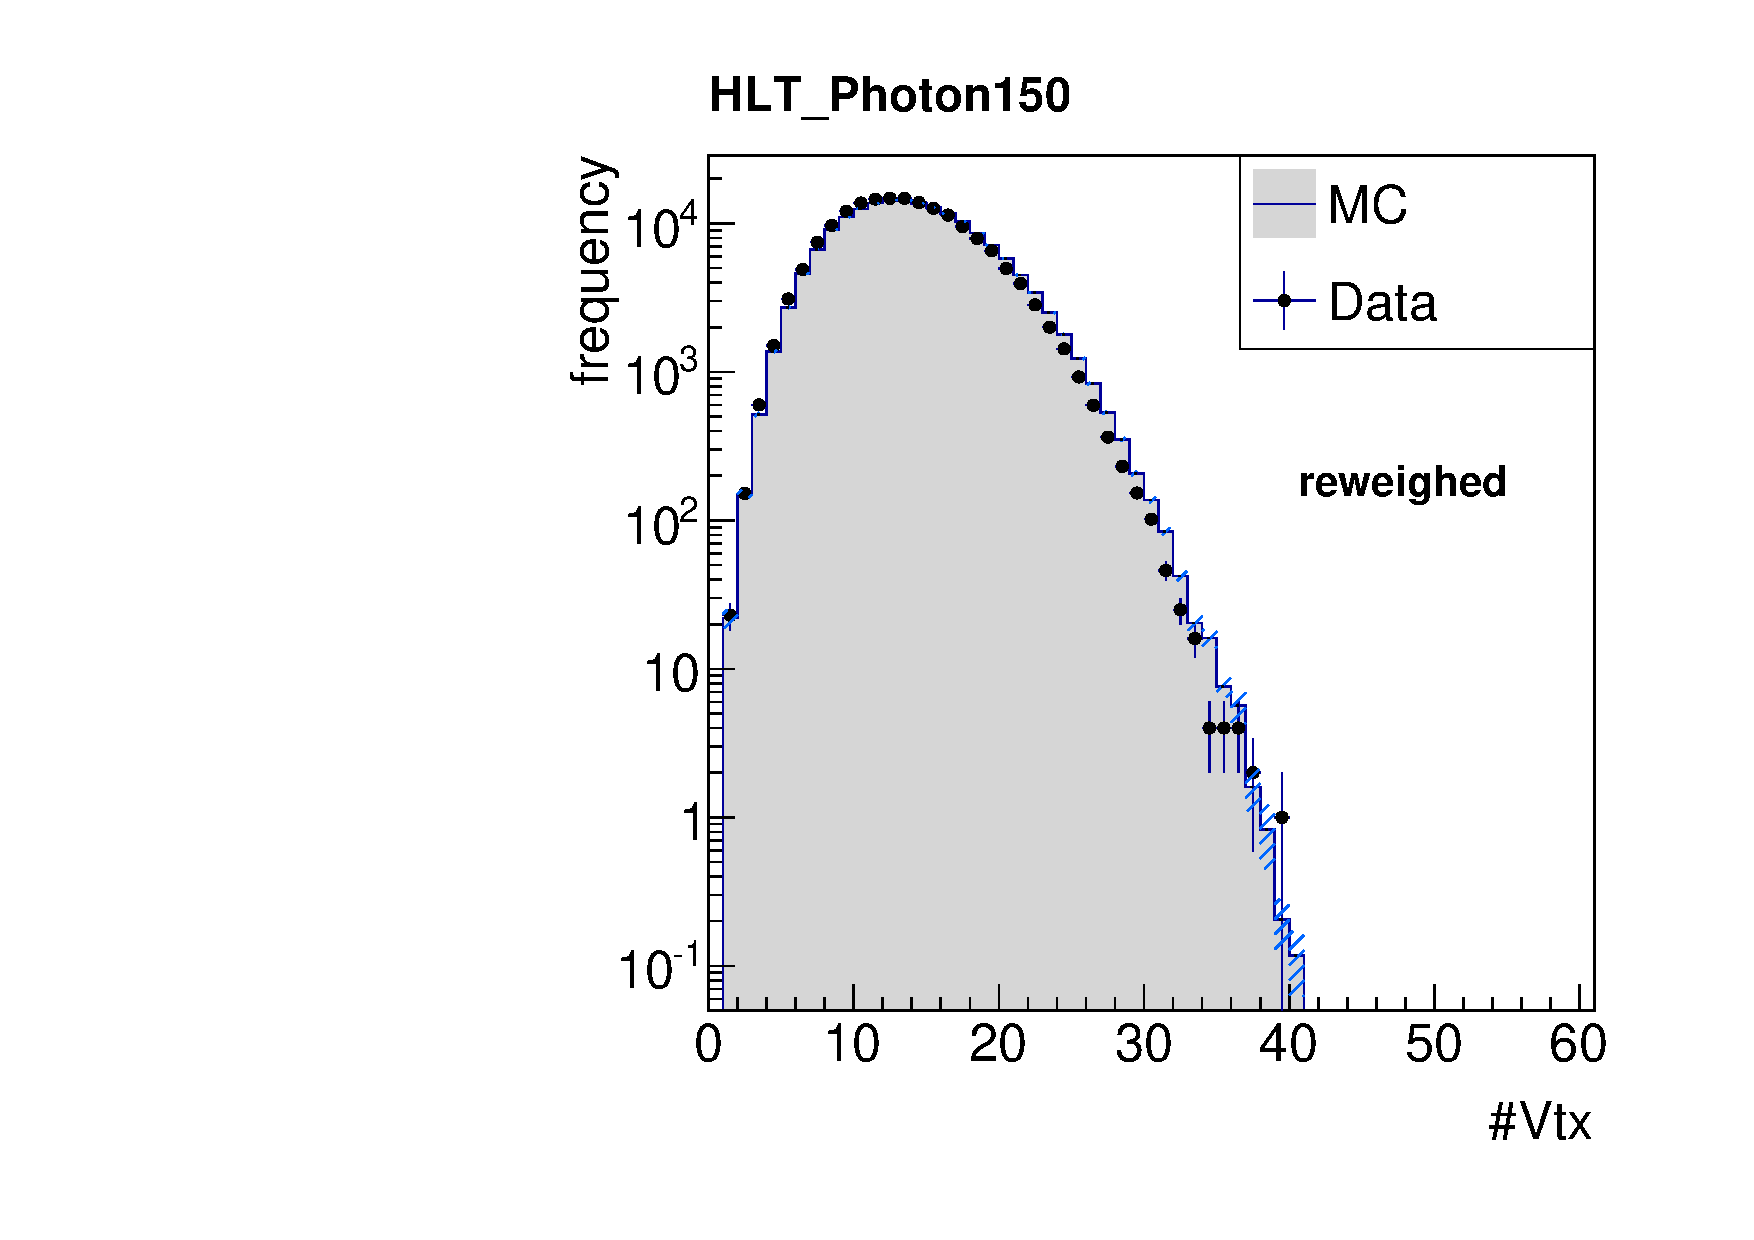
\includegraphics[width=0.49\textwidth]{figures/resolution/eventSelection/NVtxComparison6.pdf} 
  \caption{The number of primary vertices in data and simulation before (left) and after (right) reweighing for all events with $\pt^{\gamma}>165\gev$.}  
 \label{res:fig:PUreweighing}
\end{figure}


\section{Event selection}
\label{res:sec:EventSelection}
Events were reconstructed with the particle-flow reconstruction algorithm, which uses information of all detector components to reconstruct individual particles \cite{CMS-PAS-PFT-09-001}.
Furthermore, particles belonging to a jet were clustered with the Anti-k$_{\text{t}}$ jet clustering algorithm with a radius of \mbox{R=0.5 \cite{Cacciari:2008gp}.}

To select clean \GAMJET events, it was required that 
the leading jet meets the following requirements (these criteria correspond to a 'tight ID' in \cite{website:JetIdentification,CMS-AN-2010-003}):
\begin{itemize}

 \item Neutral hadron fraction $<$ 0.90
 \item Neutral electromagnetic fraction $<$ 0.90
 \item Number of constituents $>$ 1
\end{itemize}

 And for jets in the pseudorapidity range $|\eta^{\text{jet}}| < 2.4 $ :
\begin{itemize}
 \item Charged hadron fraction $>$ 0
 \item Charged hadron multiplicity $>$ 0
 \item Charged electromagnetic fraction $<$ 0.99
\end{itemize}

To mitigate effects from pileup, the first and second jet were required to have a transverse momentum greater \mbox{10\gev}.

Concerning the photon, a maximal pseudorapidity of the photon of $|\eta^{\gamma}| < 1.3$ was demanded to exploit the high resolution of the ECAL in the barrel region.

Furthermore, the resolution was determined for different ranges in photon \pt to avoid mixing of different prescales of the various triggers. 
In \mbox{Table \ref{res:tab:PhotonPtBins}} the applied binning is shown with the respective triggers contributing to each $\pt^{\gamma}$ bin.

\begin{table}[htb]
\caption{Photon \pt bins and corresponding triggers.}
\renewcommand{\arraystretch}{1.5}
\begin{center}
\begin{tabular}{ l| c }
$\pt^{\gamma}$-bins           & Trigger       \\\hline
22\gev    & \texttt{HLT\_Photon20\_CaloIdVL\_IsoL\_v*}    \\\hline
36\gev    & \texttt{HLT\_Photon30\_CaloIdVL\_IsoL\_v*}     \\\hline
60\gev    & \texttt{HLT\_Photon50\_CaloIdVL\_IsoL\_v*} \\\hline
88\gev    & \texttt{HLT\_Photon75\_CaloIdVL\_IsoL\_v*} \\\hline
105\gev   & \texttt{HLT\_Photon90\_CaloIdVL\_IsoL\_v*} \\\hline
149\gev & \texttt{HLT\_Photon135\_v*}       \\\hline
165\gev   & \texttt{HLT\_Photon150\_v*}       \\\hline
\end{tabular}
\end{center}
\label{res:tab:PhotonPtBins}
\end{table}

QCD multijets events constitute an important background to the \GAMJET events: A photon can be faked by a $\pi^{0}$ decaying into two close-by photons. 
Therefore, a very clean selection of the photons is necessary to suppress this background.
The following variables were used (see \cite{CMS-PAS-EGM-10-006} for further explanation of the variables):

\begin{itemize}
 \item $\boldmath{\frac{\textbf{H}}{\textbf{E}}}$ : The ratio of the measured energy in the hadronic calorimeter over the energy measured in the electromagnetic calorimeter. 
                                                    For photons, this is supposed to be very small as they deposit their energy predominantly in the ECAL.
 \item $\boldmath{\sigma_{i\eta i \eta}}$: The energy weighted spatial width of the photon energy deposition. The electromagnetic shower of a photon has a small lateral size 
                                           resulting in small $\sigma_{i\eta i \eta}$ for prompt photons while showers from fake photons, \eg $\pi^{0} \rightarrow \gamma \gamma$
                                           have a larger lateral size.
 \item \textbf{Jurassic ECAL isolation}: This isolation criterion uses the information of reconstructed hits ``RecHits'' (coming from the local reconstruction of the digital signals) 
                                         in a cone around the photon supercluster of R=0.4. Those are summed up and an upper criterion is identified to discriminate against 
                                         background which is typically spatially broader.  
 \item \textbf{Tower-based HCAL isolation}: The isolation criterion requires the energy deposited in all HCAL towers around the photon in cone of R=0.4 to be small compared to the 
                                            photon's energy. 
 \item \textbf{Hollow cone track isolation}: Requires absence of high-energetic tracks around the photon.
 \item \textbf{Pixel seed veto}: In order to reduce the background from electrons and positrons, the absence of a pixel-seed in the pixel tracker along the photons 
                                 trajectory is required.
\end{itemize}

The upper and lower bounds for the various requirements can be found in table \ref{res:tab:PhotonIsolation}. 

%\begin{table}[bt]
%\caption{Upper and lower bounds for all photon isolation criteria in the barrel $\left( |\eta^{\gamma}|<1.4442 \right)$ and endcap $\left(1.4442 <|\eta^{\gamma}|<2.5 \right)$ .}
%\renewcommand{\arraystretch}{1.5}
%\begin{center}
%\begin{tabular}{ l| c | c |}
%                              & Barrel                                  & Endcap                                  \\\hline
%$\frac{\text{H}}{\text{E}}$   & $<$ 0.05                                & $<$ 0.05                                \\\hline
%$\sigma_{i\eta i \eta}$       & $<$ 0.013                               & $<$ 0.03                                \\\hline
%ECAL isolation                & $<4.2 + 0.0060 \, \pt^{\gamma}$   & $<4.2 + 0.0060 \, \pt^{\gamma}$    \\\hline
%HCAL isolation                & $<2.2 + 0.0025 \, \pt^{\gamma}$   & $<2.2 + 0.0025 \, \pt^{\gamma}$   \\\hline
%Track Isolation               & $<2.0 + 0.0010 \, \pt^{\gamma}$   & $<2.0 + 0.0010 \, \pt^{\gamma}$    \\\hline
%Pixel seed veto               & yes                                     & yes                                     \\\hline
%\end{tabular}
%\end{center}
%\label{tab:PhotonIsolation}
%\end{table}

\begin{table}[bt]
\caption{Upper and lower bounds for all photon isolation criteria in the barrel $\left( |\eta^{\gamma}|<1.4442 \right)$.}
\renewcommand{\arraystretch}{1.5}
\begin{center}
\begin{tabular}{ l| c |}
                              & Barrel                            \\\hline
$\frac{\text{H}}{\text{E}}$   & $<$ 0.05                          \\\hline
$\sigma_{i\eta i \eta}$       & $<$ 0.013                         \\\hline
ECAL isolation                & $<4.2 + 0.0060 \, \pt^{\gamma}$   \\\hline
HCAL isolation                & $<2.2 + 0.0025 \, \pt^{\gamma}$   \\\hline
Track Isolation               & $<2.0 + 0.0010 \, \pt^{\gamma}$   \\\hline
Pixel seed veto               & yes                               \\\hline
\end{tabular}
\end{center}
\label{res:tab:PhotonIsolation}
\end{table}

Besides the mentioned requirements concerning the objects' attributes, two further criteria related to the event topology are crucial for this analysis:\\
An upper threshold on $\Delta \Phi$ between the leading jet and 
the photon and a maximal value for $\alpha$
\begin{itemize}

 \item $\Delta \Phi \left(\text{1st jet}, \gamma \right) > 2.95\unit{rad}$
 \item $\frac{\pt^{\text{2nd jet}}}{\pt^{\gamma}} < 0.20$.

\end{itemize}
These requirements are important to suppress events with too much further hadronic activity.

A summary of all selection criteria can be found in appendix \ref{res:app:eventselection}.


Pictures as root file available:
\begin{itemize}
\item BLA
\end{itemize}

Picture \textcolor{red}{NOT} as root file available:
\begin{itemize}
\item BLA
\end{itemize}
%%%%%%%%%%%%%%%%%%%%%%%%%%%%%%%%%%%%%%%%%%%%%%%%%%%%%%%%%%%%%%%%%%%%%%%%%%%%%%%%%%%%%%%%%%%%%%%%%%%%%%%%%%%%%%%%%%%%%%%%%%%%%%%%%%%%%%%%%%%%%%%%%%%%%%%%%%%%%%%%%%%%%%%%%%%%%%%%%%%%%%%%%%%%%%%%%%%%%%%%%%%%%%%%%%%%%%%%%%%%%%%%%%%%%%%%%%%

%%%%%%%%%%%%%%%%%%%%%%%%%%%%%%%%%%%%%%%%%%%%%%%%%%%%%%%%%%%%%%%%%%%%%%%%%%%%%%%%%%%%%%%%%%%%%%%%%%%%%%%%%%%%%%%%%%%%%%%%%%%%%%%%%%%%%%%%%%%%%%%%%%%%%%%%%%%%%%%%%%%%%%%%%%%%%%%%%%%%%%%%%%%%%%%%%%%%%%%%%%%%%%%%%%%%%%%%%%%%%%%%%%%%%%%%%%%
%%%%%%%%%%%%%%%%%%%%%%%%%%%%%%%%%%%%%%%%%%%%%%%%%%%%%%%%%%%%%%%%%%%%%%%%%%%%%%%%%%%%%%%%%%%%%%%%%%%%%%%%%%%%%%%%%%%%%%%%%%%%%%%%%%%%%%%%%%%%%%%%%%%%%%%%%%%%%%%%%%%%%%%%%%%%%%%%%%%%%%%%%%%%%%%%%%%%%%%%%%%%%%%%%%%%%%%%%%%%%%%%%%%%%%%%%%%
\chapter{Methodology of the measurement}

\begin{itemize}
\item Take from AN
\end{itemize}

Pictures as root file available:
\begin{itemize}
\item BLA
\end{itemize}

Picture \textcolor{red}{NOT} as root file available:
\begin{itemize}
\item BLA
\end{itemize}
%%%%%%%%%%%%%%%%%%%%%%%%%%%%%%%%%%%%%%%%%%%%%%%%%%%%%%%%%%%%%%%%%%%%%%%%%%%%%%%%%%%%%%%%%%%%%%%%%%%%%%%%%%%%%%%%%%%%%%%%%%%%%%%%%%%%%%%%%%%%%%%%%%%%%%%%%%%%%%%%%%%%%%%%%%%%%%%%%%%%%%%%%%%%%%%%%%%%%%%%%%%%%%%%%%%%%%%%%%%%%%%%%%%%%%%%%%%

%%%%%%%%%%%%%%%%%%%%%%%%%%%%%%%%%%%%%%%%%%%%%%%%%%%%%%%%%%%%%%%%%%%%%%%%%%%%%%%%%%%%%%%%%%%%%%%%%%%%%%%%%%%%%%%%%%%%%%%%%%%%%%%%%%%%%%%%%%%%%%%%%%%%%%%%%%%%%%%%%%%%%%%%%%%%%%%%%%%%%%%%%%%%%%%%%%%%%%%%%%%%%%%%%%%%%%%%%%%%%%%%%%%%%%%%%%%
%%%%%%%%%%%%%%%%%%%%%%%%%%%%%%%%%%%%%%%%%%%%%%%%%%%%%%%%%%%%%%%%%%%%%%%%%%%%%%%%%%%%%%%%%%%%%%%%%%%%%%%%%%%%%%%%%%%%%%%%%%%%%%%%%%%%%%%%%%%%%%%%%%%%%%%%%%%%%%%%%%%%%%%%%%%%%%%%%%%%%%%%%%%%%%%%%%%%%%%%%%%%%%%%%%%%%%%%%%%%%%%%%%%%%%%%%%%
\chapter{Systematic uncertainties}

\begin{itemize}
\item difficult to take from AN
\end{itemize}

Pictures as root file available:
\begin{itemize}
\item BLA
\end{itemize}

Picture \textcolor{red}{NOT} as root file available:
\begin{itemize}
\item BLA
\end{itemize}
%%%%%%%%%%%%%%%%%%%%%%%%%%%%%%%%%%%%%%%%%%%%%%%%%%%%%%%%%%%%%%%%%%%%%%%%%%%%%%%%%%%%%%%%%%%%%%%%%%%%%%%%%%%%%%%%%%%%%%%%%%%%%%%%%%%%%%%%%%%%%%%%%%%%%%%%%%%%%%%%%%%%%%%%%%%%%%%%%%%%%%%%%%%%%%%%%%%%%%%%%%%%%%%%%%%%%%%%%%%%%%%%%%%%%%%%%%%

%%%%%%%%%%%%%%%%%%%%%%%%%%%%%%%%%%%%%%%%%%%%%%%%%%%%%%%%%%%%%%%%%%%%%%%%%%%%%%%%%%%%%%%%%%%%%%%%%%%%%%%%%%%%%%%%%%%%%%%%%%%%%%%%%%%%%%%%%%%%%%%%%%%%%%%%%%%%%%%%%%%%%%%%%%%%%%%%%%%%%%%%%%%%%%%%%%%%%%%%%%%%%%%%%%%%%%%%%%%%%%%%%%%%%%%%%%%
%%%%%%%%%%%%%%%%%%%%%%%%%%%%%%%%%%%%%%%%%%%%%%%%%%%%%%%%%%%%%%%%%%%%%%%%%%%%%%%%%%%%%%%%%%%%%%%%%%%%%%%%%%%%%%%%%%%%%%%%%%%%%%%%%%%%%%%%%%%%%%%%%%%%%%%%%%%%%%%%%%%%%%%%%%%%%%%%%%%%%%%%%%%%%%%%%%%%%%%%%%%%%%%%%%%%%%%%%%%%%%%%%%%%%%%%%%%
\chapter{Results}

\begin{itemize}
\item THINK
\end{itemize}

Pictures as root file available:
\begin{itemize}
\item BLA
\end{itemize}

Picture \textcolor{red}{NOT} as root file available:
\begin{itemize}
\item BLA
\end{itemize}
%%%%%%%%%%%%%%%%%%%%%%%%%%%%%%%%%%%%%%%%%%%%%%%%%%%%%%%%%%%%%%%%%%%%%%%%%%%%%%%%%%%%%%%%%%%%%%%%%%%%%%%%%%%%%%%%%%%%%%%%%%%%%%%%%%%%%%%%%%%%%%%%%%%%%%%%%%%%%%%%%%%%%%%%%%%%%%%%%%%%%%%%%%%%%%%%%%%%%%%%%%%%%%%%%%%%%%%%%%%%%%%%%%%%%%%%%%%

%%%%%%%%%%%%%%%%%%%%%%%%%%%%%%%%%%%%%%%%%%%%%%%%%%%%%%%%%%%%%%%%%%%%%%%%%%%%%%%%%%%%%%%%%%%%%%%%%%%%%%%%%%%%%%%%%%%%%%%%%%%%%%%%%%%%%%%%%%%%%%%%%%%%%%%%%%%%%%%%%%%%%%%%%%%%%%%%%%%%%%%%%%%%%%%%%%%%%%%%%%%%%%%%%%%%%%%%%%%%%%%%%%%%%%%%%%%
%%%%%%%%%%%%%%%%%%%%%%%%%%%%%%%%%%%%%%%%%%%%%%%%%%%%%%%%%%%%%%%%%%%%%%%%%%%%%%%%%%%%%%%%%%%%%%%%%%%%%%%%%%%%%%%%%%%%%%%%%%%%%%%%%%%%%%%%%%%%%%%%%%%%%%%%%%%%%%%%%%%%%%%%%%%%%%%%%%%%%%%%%%%%%%%%%%%%%%%%%%%%%%%%%%%%%%%%%%%%%%%%%%%%%%%%%%%
\chapter{Discussion and conclusion}

\begin{itemize}
\item Repeat results
\item cross-check analysis
\item Outlook
\end{itemize}

Pictures as root file available:
\begin{itemize}
\item BLA
\end{itemize}

Picture \textcolor{red}{NOT} as root file available:
\begin{itemize}
\item BLA
\end{itemize}
